% TODO mention what is for best wiki and what essential

\section{Collaboration with the Creativity/Design Team \index{Design}} \label{sec:2.1}
To create an effective and visually appealing iGEM Wiki, collaboration with the Creativity/Design team is essential.
You do not only want to simply collect information on your wiki, but present it in a coherent, readable and convincing way to both fellow iGEMers and judges.
Consider the following design aspects:

\paragraph{Choosing Colors:} Select a cohesive color palette that reflects your team’s branding.\\
If the team has no prior experience with design, \href{https://en.wikipedia.org/wiki/Color_psychology}{color psychology}\cite{colorpsychology} or simply color palette choosing tools can be a helpful starting point, especially in small teams with limited resources.
\paragraph{Initial Design Work:} Ideally, start in a design program or layout tool (e.g.\ Figma) to visualize your ideas before implementing them on the Wiki.
Alternatively, vision boards or analogue planning methods such as drawing work as well.
\paragraph{Choosing Illustration Styles:} Decide on illustration styles that align with your overall design and branding.
Consistency in style helps create a unified look across your Wiki, making it more visually appealing and easier for users to navigate. \\
Style considerations can be the software used for illustrations and specific details such as the usage of borders and shadows for in-house designs.
\begin{figure}[H]
    \centering
    \begin{subfigure}[t]{0.3\linewidth}
        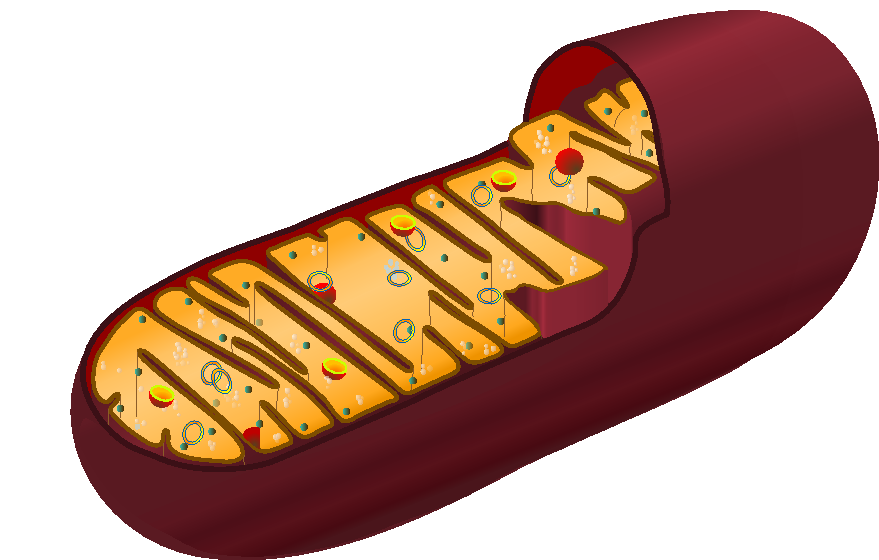
\includegraphics[width=\textwidth]{chapters/images/animal_mitochondrion}
    \end{subfigure}
    \begin{subfigure}[t]{0.3\linewidth}
        
\includegraphics[width=\textwidth]{chapters/images/mitochondrium-rod}
    \end{subfigure}
    \begin{subfigure}[t]{0.3\linewidth}
        
\includegraphics[width=\textwidth]{chapters/images/mitochondrium-servier}
    \end{subfigure}
    \caption{Different styles.}
    \label{fig:diff-styles}
    % evtl. https://reserve.freesvg.org/mitochondria
\end{figure}
\begin{figure}[H]
    \centering
    \begin{subfigure}[t]{0.2\linewidth}
        
\includegraphics[width=\textwidth]{chapters/images/mitochondria-black-lines}
    \end{subfigure}
    \begin{subfigure}[t]{0.2\linewidth}
        
\includegraphics[width=\textwidth]{chapters/images/mitochondria-yellow}
    \end{subfigure}
    \begin{subfigure}[t]{0.2\linewidth}
        
\includegraphics[width=\textwidth]{chapters/images/mitochondria-no-lines}
    \end{subfigure}
    \begin{subfigure}[t]{0.2\linewidth}
        
\includegraphics[width=\textwidth]{chapters/images/mitochondria-color-lines}
    \end{subfigure}
    \begin{subfigure}[t]{0.2\linewidth}
        
\includegraphics[width=\textwidth]{chapters/images/mitochondria-only-lines}
    \end{subfigure}
    \begin{subfigure}[t]{0.2\linewidth}
        
\includegraphics[width=\textwidth]{chapters/images/mitochondria-greyscale}
    \end{subfigure}
    \caption{How different basic styles.}
    \label{fig:basic-styles}
\end{figure}

%\paragraph{Importance of Branding:} Establish a strong brand identity through consistent use of colors and design elements.
\paragraph{Logo usage:} There are many possibilities to use your team logo on your wiki.
Both for simple things such as buttons as well as more complex things such as animations, progress bars or a guide through your website.
% TODO images or links of examples

\section{Design Parameters} \label{sec:design-paramaters} \index{Design}
\begin{itemize}
    \item \textbf{Typography:} Prioritize typography to enhance readability and aesthetics.
    \begin{itemize}
        \item Maintain appropriate line length and spacing for readability.
        \item Use standardized font sizes for consistency across the Wiki.
    \end{itemize}
    \item \textbf{Simplicity:} Aim to simplify designs for a cleaner look.
    \begin{itemize}
        \item Limit to 2--3 headings and colors to maintain clarity and focus.
        \item Minimize the number of design parameters to streamline the design process.
        \item Use colors purposefully; avoid unnecessary embellishments unless justified.
    \end{itemize}
    \item \textbf{Consistency:} Unify illustration styles and design elements for a cohesive appearance.
    \begin{itemize}
        \item Ensure consistent image formats and alignment (preferably left-aligned, avoiding justified text).
        \item Align infographic styles to maintain a cohesive visual narrative.
    \end{itemize}
    \item \textbf{Bootstrap Values:} Consider overriding Bootstrap defaults as needed for your design (See \nameref{sec:bootstrap}).
    \item \textbf{Call to action and clear navigation:} Include a welcoming call to action on the homepage, using colors meaningfully to guide users.
    \begin{itemize}
        \item Possibly add further guidance such as highlights, to guide the user through the wiki and help the judges find all necessary information.
        \item Use a clear menu structure and possibly breadcrumbs.
        \item Avoid deep nesting your pages and aim for a flat, user-friendly structure.
        You want the judges to easily find all you pages from the standard URLs.
    \end{itemize}
    \item \textbf{Content Organization:} Clear information hierarchy helps users find what they’re looking for faster.
    \begin{itemize}
        \item Utilize cards or expandable sections for content organization.
        \item Ensure the basic information is always available and additional information is, while easily locatable, tucked away and not distracting the reader.
    \end{itemize}
\end{itemize}
\begin{itemize}
    \item \textbf{Responsiveness:} Ensure that all design elements adapt smoothly to different screen sizes (See \nameref{sec:bootstrap}).
    \begin{itemize}
        \item Prioritize mobile usability since people may want to look at your wiki on their phones during or after presentations and poster sessions.
        \item Verify that navigation, text, and visuals remain accessible and visually consistent across devices.
    \end{itemize}
    \item \textbf{Accessibility:} Design for inclusivity by ensuring content is accessible to all users.
    Especially if you aim for the inclusivity special prize. \index{special prize!inclusivity}
    \begin{itemize}
        \item Maintain sufficient color contrast for readability.
        \item Use semantic HTML and alt text for images.
    \end{itemize}
\end{itemize}
